\label{Section:FISSC}
FISSC\footnote{FISSC hyperlink: \href{https://hal.science/hal-03784107v1/file/article-fissc.pdf}{https://hal.science/hal-03784107v1/file/article-fissc.pdf}} (Fault Injection and Simulation Secure Collection) is a public code collection dedicated to the analysis of code robustness against fault injection attacks. It contains two pieces of code that we will discuss in this section:
\begin{itemize}
\item The first code evaluated is \texttt{verify\_pin}, a program used to validate a PIN code on a PIN pad.
\item The second code is \texttt{memcmps}, a secure version of \texttt{memcmp}.
\end{itemize}
Originally written in C, both code segments were ported to Rust, following a C-style programming approach, and were subsequently examined using Lazart. Then, each code in both languages was analyzed and compared.
In addition to the comparison, we have also written a more idiomatic version of the FISSC collection.

%--------------------------------------------------------------verifypin--------------------------------------------------------------------------------
\subsection{\textit{verifypin} collection}

\begin{figure}[ht]
    \centering
    \fbox{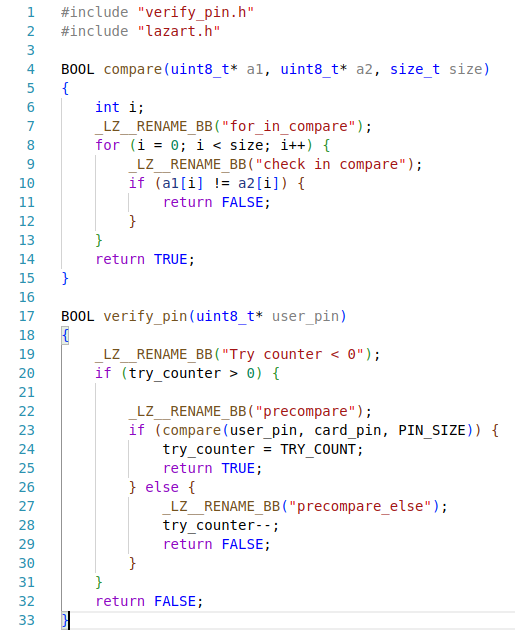
\includegraphics[scale=0.35]{image/verify_pin_0_C.png}}
    \caption{Verification of PIN code in C}
    \label{figure 3 : verifypin_C}
\end{figure}

The second example code implemented in Rust is \textbf{verifypin}.\\
The \texttt{verify\_pin} program implements the PIN verification process of a smart card.\\
The source code in C shown in Figure \ref{figure 3 : verifypin_C} corresponds to a simple implementation without countermeasures other than a hardened boolean.

The \textbf{verifypin} function consists of two parts:
\begin{itemize}
    \item Checking if there are enough tries remaining (line 20 in Figure \ref{figure 3 : verifypin_C}).
    \item Resetting the try counter and returning \texttt{TRUE} if the \texttt{compare} function returns \texttt{TRUE}; otherwise, decrementing the number of tries remaining by 1 and returning \texttt{FALSE}.\\
\end{itemize}

\noindent\texttt{\textbf{TRUE}} contains the value \texttt{0xAA}.\\
\texttt{\textbf{FALSE}} contains the value \texttt{0x55}.\\

We consider \texttt{TRUE} and \texttt{FALSE} as hardened boolean values because they are encoded not just as single 0 or 1 bits, but as 8-bit patterns of 0s and 1s. Specifically, the pattern ‘01’ represents \texttt{FALSE}, while ‘10’ represents \texttt{TRUE}.\\
This approach makes it highly unlikely for a \texttt{TRUE} value to be accidentally flipped to \texttt{FALSE}, or vice versa.

The function takes one user PIN and returns either \texttt{TRUE} or \texttt{FALSE}.

The function \textbf{compare}, shown in Figure \ref{figure 3 : verifypin_C}, compares each digit of the user input PIN with the one stored on the card.
It returns \texttt{TRUE} if both PIN codes are identical and \texttt{FALSE} otherwise.

We studied two attack objectives with the help of an oracle:
\begin{itemize}
    \item Returning \texttt{TRUE} when both PIN codes are different.
    \item Increasing the number of tries remaining in the case where both PIN codes are different.
\end{itemize}

The attack model used is the \textbf{test inversion}.

We implemented the Rust version of the source code shown in Figure \ref{figure 3 : verifypin_C}, following the style used by C programmers (see Figure \ref{figure 4 : verifypin_Rust}).



%--------------------------------------------------------------memcmps--------------------------------------------------------------------------------
\subsection{\textit{memcmps} collection}

\begin{figure}[ht]
    \centering
    \fbox{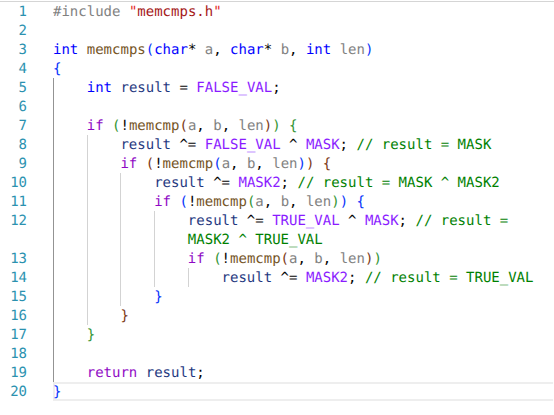
\includegraphics[scale=0.35]{image/memcmps_C.png}}
    \caption{Securised version of memcmp in C}
    \label{figure 1:memcmps_C}
\end{figure}

\begin{figure}[ht]
    \centering
    \fbox{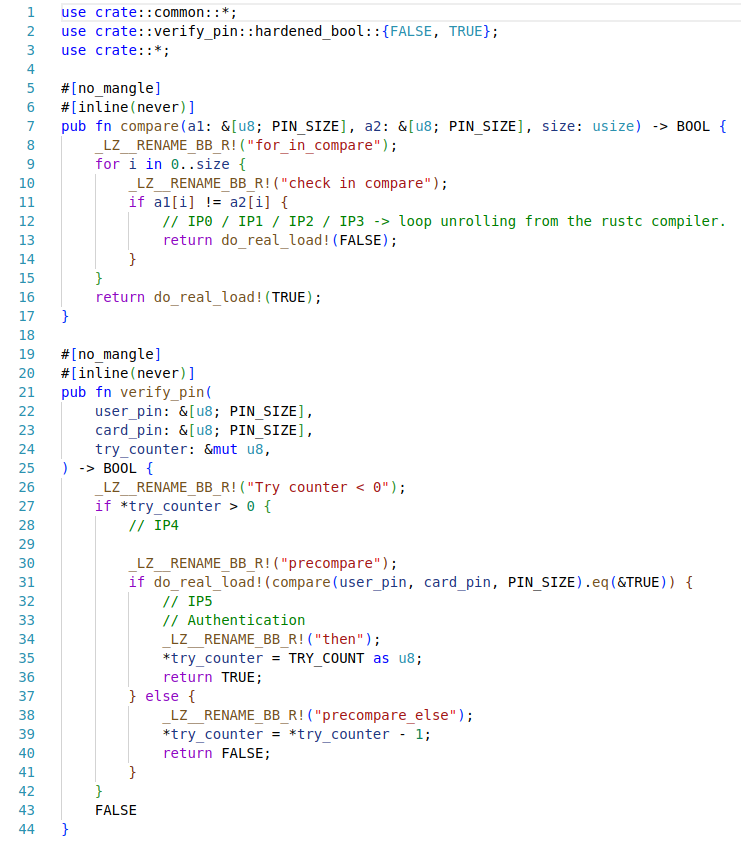
\includegraphics[scale=0.35]{image/verify_pin_0_Rust.png}}
    \caption{Verification of PIN code in Rust}
    \label{figure 4 : verifypin_Rust}
\end{figure}

The first example code implemented in Rust is \texttt{memcmps}.\\
\texttt{memcmps} is a secure version of  \texttt{memcmp}  that is available in C.\\

\texttt{memcmps} takes two input arrays that are initialized before the function is called.\\
\texttt{memcmps} returned two possible values:\\
\begin{itemize}
    \item \texttt{TRUE\_VAL}, corresponding to \texttt{0x1234}, when both arrays are equal.
    \item \texttt{FALSE\_VAL}, corresponding to \texttt{0x5678}, when they are not equal.
\end{itemize}
\vspace{0.5cm}

In Figure \ref{figure 1:memcmps_C}, we show one of the three versions of \texttt{memcmps} that we implemented.
This version used four function calls of \texttt{memcmp}  as shown in lines 7, 9, 11, and 13 and two masks, \texttt{MASK} and \texttt{MASK2}, to prevent fault injection from affecting the returned value of the function.
\begin{itemize}
    \item \texttt{MASK} corresponding to the value \texttt{0xABCD}
    \item \texttt{MASK2} corresponding to the value \texttt{0xF4F4}
\end{itemize}
\vspace{0.5cm}

\texttt{memcmps} works by using \texttt{MASK} on a variable called result (see line 5 on Figure \ref{figure 1:memcmps_C}).\\
If no fault is injected into the system, \texttt{memcmps} should return either true or false every time it is called.\\
So if both data blocks are the same, then the result will take the value of \texttt{MASK} after the first call at line 8.\\
the value take \texttt{MASK} $\land$ \texttt{MASK2} after the second call line 10.\\
the value take \texttt{MASK2} $\land$ \texttt{TRUE\_VAL} after the third call line 12.\\
And finally the value takes \texttt{TRUE\_VAL} after the fourth call line 14.\\

We studied two attack objectives with the help of an oracle:

\begin{itemize}
    \item returning \texttt{TRUE\_VAL} when both data blocks are \textbf{different}.
    \item returning anything but \texttt{FALSE\_VAL} when both data blocks are equal. 
\end{itemize}

The attack model used is the inversion test and data mutation, in the figure \ref{figure 1:memcmps_C}, one inversion test may cause the value to be neither \texttt{TRUE\_VAL} nor \texttt{FALSE\_VAL} (if the attack is done on the condition test line 7).
Four inversion tests are needed to be able to return \texttt{TRUE\_VAL} when the data blocks are different.

We implemented the Rust version of the code that would be written by C programmers.

\begin{figure*}[ht]
    \centering
    \fbox{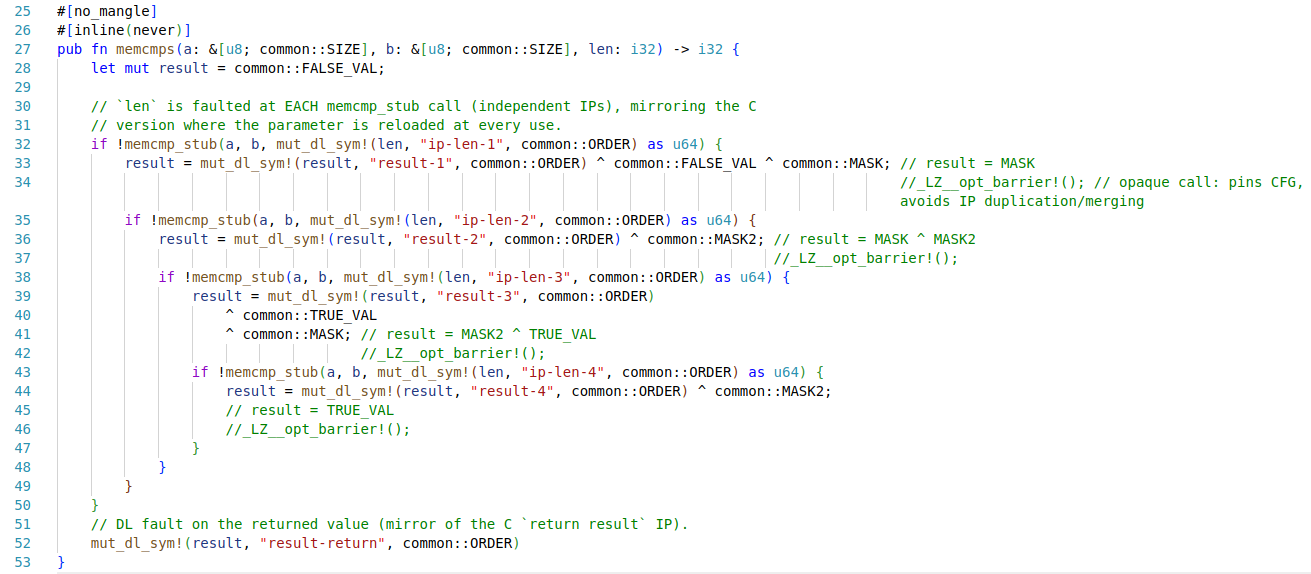
\includegraphics[scale=0.35]{image/memcmps_Rust.png}}
    \caption{Secured version of memcmp in Rust}
    \label{figure 2:memcmps_Rust}
\end{figure*}

Figure \ref{figure 2:memcmps_Rust} shows the \texttt{memcmps} source code equivalent of Figure \ref{figure 1:memcmps_C} in the Rust language.\\
In the Rust version of \texttt{memcmps}, we needed to change the return value of \texttt{memcmp}, due to C not having a native boolean type.\\
\texttt{memcmp} returns \textit{false} if both binary data blocks are the same and \textit{true} otherwise.\\
We also used two flags for compiling Rust:
\begin{itemize}
    \item The first is the use of the \texttt{no\_mangle} flag on line 17 in Figure \ref{figure 2:memcmps_Rust}.\\It is used to prevent Rust from renaming some of the blocks generated by the LLVM and to ensure the correct operation of Lazart.
    \item The second is the use of \texttt{inline(never)} on line 18, which forces Rust not to replace the function call with its body.\\ This is a type of optimization used by compilers to avoid context changes.
\end{itemize}
In memcmps programs, the data load(DL) faults are directly instrumented in the program (using \texttt{mut\_dl\_sym!} macro), instead of being specified by variable name. That prevent the propagation of the \texttt{len} value in SSA,
which the DL model applies. This also prevents the constant folding for result that is reduced to a selection of constants depending on the execution path. Thus, direct calls to the DL mutation macro are made on each DL injection point.
%-------------------------------------idiomatic-Rust-----------------------------------------------------------
\subsection{A Rust version FISSC}
\todo[inline]{I or we ?}
I developed an idiomatic version of FISSC in Rust. The idiomatic version contain both previous examples, \texttt{verify\_pin} and \texttt{memcmps}.
Unlike the two previous examples, the goal is not to match one-to-one the C implementation but to provide a collection of code that can be reused with other formal-methods or simulation tools, or on another representation level.
In addition to the idiomatic Rust versions of \texttt{verify\_pin} and \texttt{memcmps} collections, we ported the remaining programs of FISSC to Rust.
We briefly describe here the CRT-RSA, AES and GetChallenge programs from FISSC.

The \texttt{CRT-RSA collection} implements three versions of RSA signing using the Chinese Remainder Theorem (CRT).
The program is vulnerable to the Bellcore attack and the attack objective consists of corrupting one of the two partial results, producing an invalid signature while remaining congruent to it modulo p or q. Three variants exist: Basic (unprotected), Shamir (coherence check between the two exponentiations in an extended domain p·r), and Aumüller (multiple integrity checks on parameters, output, and a cross domain check).

The two AES examples consist of the implementation of the full AES cipher and the isolated AES AddRoundKey step. The program's attack objective is to generate an invalid ciphertext.

The \textit{Get Challenge collection} (GC) corresponds to the generation of a random challenge in an authentication protocol. The program's attack objective is to set the flag to \texttt{true} without being detected by the sentinel value in the buffer.
The hardened variant stacks four software countermeasures - virtual call stack, doubled arguments, step counter, and loop counter.